\documentclass[../../main/main.tex]{subfiles}
\graphicspath{{./figures/}}
\usepackage{custikz}

\dominitoc
\faketableofcontents

\renewcommand{\mtcSfont}{\small\bfseries}
\renewcommand{\mtcSSfont}{\footnotesize}
\mtcsettitle{minitoc}{}
\mtcsetrules{*}{off}

\makeatletter
\renewcommand{\@chapapp}{Thermodynamique -- chapitre}
\makeatother

% \toggletrue{student}
% \toggletrue{corrige}
% \renewcommand{\mycol}{black}
% \renewcommand{\mycol}{gray}

\hfuzz=5.003pt

\begin{document}
\setcounter{chapter}{4}

\settype{book}
\settype{prof}
\settype{stud}

\chapter{Machines thermiques}
\epigraph{\openquote\textit{%
		Thermodynamics is a funny subject. The first time you go through it, you
		don't understand it at all. The second time you go through it, you think you
		understand it, except for one or two small points. The third time you go
		through it, you know you don't understand it, but by that time you are so
		used to it, it doesn't bother you anymore.
	}%
	\closequote}{Arnold \textsc{Sommerfeld}, $\approx$ 1950}

\vspace*{\fill}

\begin{tcn}*(appl)<ctc>{\iconsomm~Sommaire}
	\let\item\olditem
	\vspace{-15pt}
	\minitoc
	\vspace{-25pt}
\end{tcn}

\begin{tcn}*[fontupper=\small](appl)<ctb>"how"'t'{Capacités exigibles}
	\begin{itemize}[label=\rcheck]
		\item Donner le sens des échanges énergétiques pour un moteur ou un
		      récepteur thermique ditherme.

		\item Analyser un dispositif concret et le modéliser par une machine
		      cyclique ditherme.

		\item Définir un rendement ou une efficacité et les relier aux énergies
		      échangées au cours d'un cycle.

		\item Justifier et utiliser le théorème de Carnot.

		\item Citer quelques ordres de grandeur des rendements des machines
		      thermiques réelles actuelles.

		\item Expliquer le principe de la cogénération.
	\end{itemize}
\end{tcn}

\vspace*{\fill}

\newpage

\vspace*{\fill}
% {
% \begin{boxes}
\begin{tcn}[sidebyside, fontupper=\small, fontlower=\small](appl)<ctb>"check"'t'{L'essentiel}
	\begin{tcn}(defi)<ctc>'t'{Définitions}
		\tcblistof[\paragraph*]{defi}{\hspace*{4.8pt}}
	\end{tcn}
	% \begin{tcn}(rapp)<ctc>'t'{Rappels}
	% 	\tcblistof[\paragraph*]{rapp}{\hspace*{4.8pt}}
	% \end{tcn}
	\begin{tcn}(prop)<ctc>'t'{Propriétés}
		\tcblistof[\paragraph*]{prop}{\hspace*{4.8pt}}
		\tcblistof[\paragraph*]{loi}{\hspace*{4.8pt}}
		% \tcblistof[\paragraph*]{theo}{\hspace*{4.8pt}}
	\end{tcn}
	% \begin{tcn}(coro)<ctc>'t'{Corollaires}
	%   \tcblistof[\paragraph*]{coro}{\hspace*{4.8pt}}
	% \end{tcn}
	\begin{tcn}(demo)<ctc>'t'{Démonstrations}
		\tcblistof[\paragraph*]{demo}{\hspace*{4.8pt}}
		\tcblistof[\paragraph*]{prev}{\hspace*{4.8pt}}
	\end{tcn}
	% \begin{tcn}(inte)<ctc>'t'{Interprétations}
	% 	\tcblistof[\paragraph*]{inte}{\hspace*{4.8pt}}
	% \end{tcn}
	% \begin{tcn}(impl)<ctc>'t'{Implications}
	% 	\tcblistof[\paragraph*]{impl}{\hspace*{4.8pt}}
	% \end{tcn}
	% \begin{tcn}(tool)<ctc>'t'{Outils}
	% 	\tcblistof[\paragraph*]{tool}{\hspace*{4.8pt}}
	% \end{tcn}
	% \begin{tcn}(nota)<ctc>'t'{Notations}
	%   \tcblistof[\paragraph*]{nota}{\hspace*{4.8pt}}
	% \end{tcn}
	% \begin{tcn}(appl)<ctc>'t'{Applications}
	%   \tcblistof[\paragraph*]{appl}{\hspace*{4.8pt}}
	% \end{tcn}
	% \begin{tcn}(rema)<ctc>'t'{Remarques}
	%   \tcblistof[\paragraph*]{rema}{\hspace*{4.8pt}}
	% \end{tcn}
	% \begin{tcn}(exem)<ctc>'t'{Exemples}
	%   \tcblistof[\paragraph*]{exem}{\hspace*{4.8pt}}
	% \end{tcn}
	% \begin{tcn}*(ror)<ctc>"hart"'t'{Points importants}
	%   \tcblistof[\paragraph*]{ror}{\hspace*{4.8pt}}
	% \end{tcn}
	% \begin{tcn}(impo)<ctc>'t'{Erreurs communes}
	%   \tcblistof[\paragraph*]{impo}{\hspace*{4.8pt}}
	% \end{tcn}
	\tcblower
	% \begin{tcn}(defi)<ctc>'t'{Définitions}
	%   \tcblistof[\paragraph*]{defi}{\hspace*{4.8pt}}
	% \end{tcn}
	% \begin{tcn}(rapp)<ctc>'t'{Rappels}
	%   \tcblistof[\paragraph*]{rapp}{\hspace*{4.8pt}}
	% \end{tcn}
	% \begin{tcn}(prop)<ctc>'t'{Propriétés}
	%   \tcblistof[\paragraph*]{prop}{\hspace*{4.8pt}}
	%   \tcblistof[\paragraph*]{loi}{\hspace*{4.8pt}}
	%   \tcblistof[\paragraph*]{theo}{\hspace*{4.8pt}}
	% \end{tcn}
	% \begin{tcn}(coro)<ctc>'t'{Corollaires}
	%   \tcblistof[\paragraph*]{coro}{\hspace*{4.8pt}}
	% \end{tcn}
	% \begin{tcn}(demo)<ctc>'t'{Démonstrations}
	% 	\tcblistof[\paragraph*]{demo}{\hspace*{4.8pt}}
	% 	\tcblistof[\paragraph*]{prev}{\hspace*{4.8pt}}
	% \end{tcn}
	\begin{tcn}(inte)<ctc>'t'{Interprétations}
		\tcblistof[\paragraph*]{inte}{\hspace*{4.8pt}}
	\end{tcn}
	% \begin{tcn}(impl)<ctc>'t'{Implications}
	% 	\tcblistof[\paragraph*]{impl}{\hspace*{4.8pt}}
	% \end{tcn}
	% \begin{tcn}(tool)<ctc>'t'{Outils}
	%   \tcblistof[\paragraph*]{tool}{\hspace*{4.8pt}}
	% \end{tcn}
	% \begin{tcn}(nota)<ctc>'t'{Notations}
	%   \tcblistof[\paragraph*]{nota}{\hspace*{4.8pt}}
	% \end{tcn}
	\begin{tcn}(odgr)<ctc>'t'{Ordres de grandeur}
		\tcblistof[\paragraph*]{odgr}{\hspace*{4.8pt}}
	\end{tcn}
	% \begin{tcn}(appl)<ctc>'t'{Applications}
	% 	\tcblistof[\paragraph*]{appl}{\hspace*{4.8pt}}
	% \end{tcn}
	% \begin{tcn}(rema)<ctc>'t'{Remarques}
	%   \tcblistof[\paragraph*]{rema}{\hspace*{4.8pt}}
	% \end{tcn}
	% \begin{tcn}(exem)<ctc>'t'{Exemples}
	% 	\tcblistof[\paragraph*]{exem}{\hspace*{4.8pt}}
	% \end{tcn}
	\begin{tcn}*(ror)<ctc>"hart"'t'{Points importants}
		\tcblistof[\paragraph*]{ror}{\hspace*{4.8pt}}
	\end{tcn}
	\begin{tcn}(impo)<ctc>'t'{Erreurs communes}
		\tcblistof[\paragraph*]{impo}{\hspace*{4.8pt}}
	\end{tcn}
\end{tcn}
% \end{boxes}
% }%

\vspace*{\fill}
\newpage

\section{Introduction}
\subsection{Définition}

\begin{tcb*}(defi){Machines thermiques et performance}
	\begin{isd}[righthand ratio=.25]
		Une machine thermique est un dispositif qui fait subir à un fluide un
		\textbf{cycle thermodynamique}, dans le but d'\textbf{extraire du travail}
		mécanique $W$ ou un \textbf{transfert thermique} $Q$.
		% Selon le type de machine, l'énergie coûteuse et l'énergie produite ne sont pas
		% les mêmes.
		\tcblower
		\tcbsubtitle{\fatbox{\textbf{Coeff.\ performance}}}
		\vspace{-15pt}
		\psw{%
			\[
				\text{COP} = \abs{\frac{\text{production}}{\text{coût}}}
			\]
		}%
		\vspace{-15pt}
	\end{isd}
	\begin{isd}[sidebyside align=top]
		\tcbsubtitle{\fatbox{\textbf{Machine motrice}}}
		Elle \textbf{fournit un travail}~:
		\begin{itemize}
			\item[b]{Production}: \psw{$W < 0$}
			\item[b]{Coût}: \psw{$Q > 0$}
			\item[b]{Rendement}\ftn{On parle de \textbf{rendement} pour un
				\textbf{moteur}, car il décrit une conversion d'énergie. On a donc
				$\eta < 1$.}: \psw{$\DS\eta = \abs{\frac{W}{Q}}$}
		\end{itemize}
		\vspace{-15pt}
		\tcblower
		\tcbsubtitle{\fatbox{\textbf{Machine réceptrice}}}
		Elle \textbf{reçoit un travail}~:
		\begin{itemize}
			\item[b]{Coût}: \psw{$W > 0$}
			\item[b]{Production}: \psw{$Q \lessgtr 0$}
			\item[b]{Efficacité}\ftn{On parle d'\textbf{efficacité} pour un
				\textbf{récepteur} puisqu'elle quantifie un transfert thermique, pas
				une conversion. On peut donc avoir $e > 1$.}: \psw{$\DS e =
					\abs{\frac{Q}{W}}$}
		\end{itemize}
		\vspace{-15pt}
	\end{isd}
\end{tcb*}
\vspace{-15pt}
\begin{tcb}(exem)<lftt>{Machines thermiques}
	\begin{itemize}
		\item Une locomotive à vapeur convertit la chaleur extraite de la cheminée
		      en mouvement des roues~: c'est un \xul{\psw{\textbf{moteur}}}.
		\item Un radiateur électrique convertit un travail électrique (effet
		      \textsc{Joule}) en chaleur~: c'est un \xul{\psw{\textbf{récepteur}}}.
		\item Un réfrigérateur récupère un travail électrique et s'en sert pour
		      capter l'énergie thermique des aliments~: c'est un
		      \xul{\psw{\text{récepteur}}}.
	\end{itemize}
\end{tcb}

\vspace{-25pt}
\subsection{Fonctionnement général}
\begin{tcb*}[sidebyside, label=prop:mchn](prop){Fonction\mnt\ des machines thermiques}
	Pour une machine en contact avec $n$ sources de chaleurs, son fonctionnement
	est régit par les \textbf{deux principes} de la thermodynamique~:
	\begin{itemize}
		\item[b]{Premier principe}:
		\psw{%
			\begin{gather}
				\Delta{U}\ind{cycle} = 0
				\Lra
				\boxed{W = -\sum_{i=1}^{n} Q_i}
				\label{eq:1ppe}
			\end{gather}
		}%
		\vspace{-15pt}
		\item[b]{Second principe} (\textbf{inégalité de \textsc{Clausius}}):
		\psw{%
			\begin{gather}
				S\ind{ech} \leq 0
				\Lra
				\boxed{\sum_{i=1}^{n} \frac{Q_i}{T_i} \leq 0}
				\label{eq:2ppe}
			\end{gather}
		}%
		\vspace{-15pt}
		% Qu'on appelle aussi \textbf{inégalité de \textsc{Clausius}}
	\end{itemize}
	\tcblower
	\begin{center}
		\sswitch{
			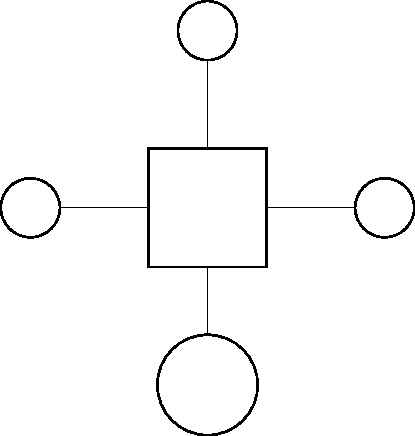
\includegraphics[scale=.8]{ppe_gen-stud}
		}{
			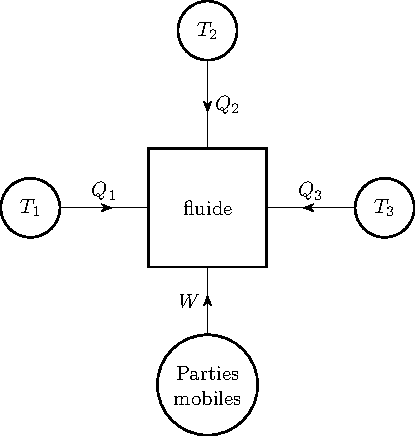
\includegraphics[scale=.8]{ppe_gen}
		}
		\captionof{figure}{Représentation des échanges}
	\end{center}
\end{tcb*}

\begin{tcb*}(impo){Échanges algébriques}
	Pour rappel, les énergies échangées sont \textbf{algébriques}, et dans le
	premier principe $W$ et $Q$ sont des énergies \textbf{reçues}~: les flèches
	sont donc dirigées \textbf{vers le fluide}, même si les échanges sont
	négatifs. On indiquera explicitement le signe des échanges pour lever la
	confusion selon le type de machine.
\end{tcb*}

\begin{tcb*}[sidebyside, sidebyside align=top](demo){Fonction\mnt\ des machines thermiques}
	\tcbsubtitle{\fatbox{\textbf{Premier principe}}}
	\vspace{-15pt}
	\psw{%
		\begin{align*}
			\Delta{U}\ind{cycle} & = 0
			\\\Lra
			W + \sum_i Q_i       & = 0
			\\\Lra
			\Aboxed{\sum_i Q_i   & = -W}
			\qed
		\end{align*}
	}%
	\vspace{-15pt}
	\tcblower
	\tcbsubtitle{\fatbox{\textbf{Inégalité de \textsc{Clausius}}}}
	\vspace{-15pt}
	\psw{%
		\begin{align*}
			\Delta{S}\ind{cycle}                                               & = 0
			\\\Lra
			\sum_i S_{\mathrm{ech},i} + \underbracket[1pt]{S\ind{cr}}_{\geq 0} & = 0
			\\\Lra
			\Aboxed{
			\sum_{i=1}^{n} \frac{Q_i}{T_i}                                     & \leq 0
			}
			\qed
		\end{align*}
	}%
	\vspace{-15pt}
\end{tcb*}

\subsection{Machines monothermes}
\begin{tcb*}[sidebyside](defi){Machine monotherme}
	Une machine thermique monotherme est composée d'un fluide en contact avec un
	\textbf{unique thermostat}.
	\tcblower
	\begin{center}
		\sswitch{
			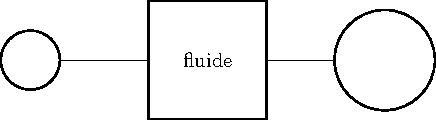
\includegraphics[width=\linewidth]{mchn_mth-stud}
		}{
			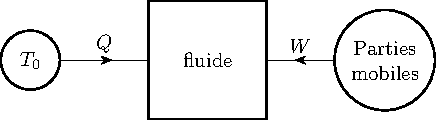
\includegraphics[width=\linewidth]{mchn_mth}
		}
		\vspace{-15pt}
		\captionof{figure}{Machine monotherme.}
	\end{center}
\end{tcb*}

\begin{tcb*}[cnt, bld](prop){Moteur monotherme}
	Il est impossible de réaliser un moteur avec une unique source de chaleur.
\end{tcb*}
\begin{tcb*}[sidebyside](demo){Moteur monotherme}
	On applique les règles de fonctionnement (Propriété~\ref{prop:mchn})~:
	\begin{gather*}
		\beforetext{1\ier{} ppe}
		\psw{%
			\Delta{U}\ind{cycle} = 0
			\Lra
			\boxed{W = -Q}
		}%
		\\\beforetext{2\up{d} ppe}
		\psw{%
			S\ind{ech} \leq 0
			\Lra
			\frac{Q}{T_0} \leq 0
		}%
		\\\beforetext{D'où}
		\psw{%
			\Ra
			Q \leq 0
			\quad \Lra \quad
			\boxed{W \geq 0}
		}%
	\end{gather*}
	\tcblower
	\begin{center}
		\sswitch{
			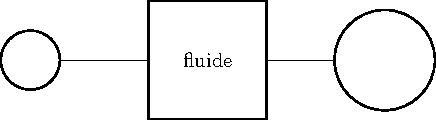
\includegraphics[width=\linewidth]{mot_mth-stud}
		}{
			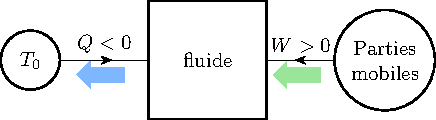
\includegraphics[width=\linewidth]{mot_mth}
		}
		\vspace{-15pt}
		\captionof{figure}{Sens des transferts.}
	\end{center}
\end{tcb*}

\begin{tcb*}(inte)<lftt>{Machine monotherme}
	Une machine monotherme est donc forcément réceptrice, et fournit un
	transfert thermique vers l'extérieur, c'est uniquement le cas pour un
	chauffage… Si on souhaite obtenir un autre type de machine thermique on a
	forcément besoin d'au moins deux thermostats.
\end{tcb*}

\section{Machines dithermes}
\subsection{Diagramme de \textsc{Raveau}}

\begin{tcb*}(defi){Machine ditherme}
	Une machine ditherme possède 2 sources de chaleur~:
	\begin{tasks}[label=\bdmd](2)
		\task \textbf{Thermostat froid}~: \psw{$T_F$ et $Q_F$~;}
		\task \textbf{Thermostat chaud}~: \psw{$T_C$ et $Q_C$.}
	\end{tasks}
\end{tcb*}

\begin{tcb*}(prop){Diagramme de \textsc{Raveau}}
	Le diagramme de \textsc{Raveau} est une visualisation permettant de voir les
	machines thermiques possibles~:
	\smallbreak
	\begin{isd}[righthand ratio=.45, fontupper=\small]
		\vspace{-15pt}
		\begin{enumerate}[label=\clenumi]
			\setlength{\fboxsep}{3mm}
			\item
			      \leftcenters{%
				      \textbf{Vert}~:
			      }{%
				      $\boxed{\psw{Q_C > 0,~Q_F < 0 \text{~et~} W < 0}}$
			      }%
			      \smallbreak
			      \psw{C'est un \xul{\textbf{moteur}}.}
			\item
			      \leftcenters{%
				      \textbf{Rouge}~:
			      }{%
				      $\boxed{\psw{Q_C > 0,~Q_F < 0 \text{~et~} W > 0}}$
			      }%
			      \smallbreak
			      \psw{%
				      C'est une machine \xul{\textbf{inutile}}, elle accélère le
				      transfert thermique du chaud vers le froid.
			      }%
			\item
			      \leftcenters{%
				      \textbf{Jaune}~:
			      }{%
				      $\boxed{\psw{Q_C < 0,~Q_F < 0 \text{~et~} W > 0}}$
			      }%
			      \smallbreak
			      \psw{%
				      C'est une machine \xul{\textbf{inutile}}, elle réchauffe les deux
				      sources.
			      }%
			\item
			      \leftcenters{%
				      \textbf{Bleu}~:
			      }{%
				      $\boxed{\psw{Q_C < 0,~Q_F > 0 \text{~et~} W > 0}}$
			      }%
			      \smallbreak
			      \psw{%
				      C'est le domaine des \xul{\textbf{réfrigérateurs}} et
				      \xul{\textbf{pompes à chaleur}}. L'inversion du sens spontané du
				      transfert thermique coûte un travail.
			      }%
		\end{enumerate}
		\vspace{-15pt}
		\tcblower
		\begin{center}
			\sswitch{
				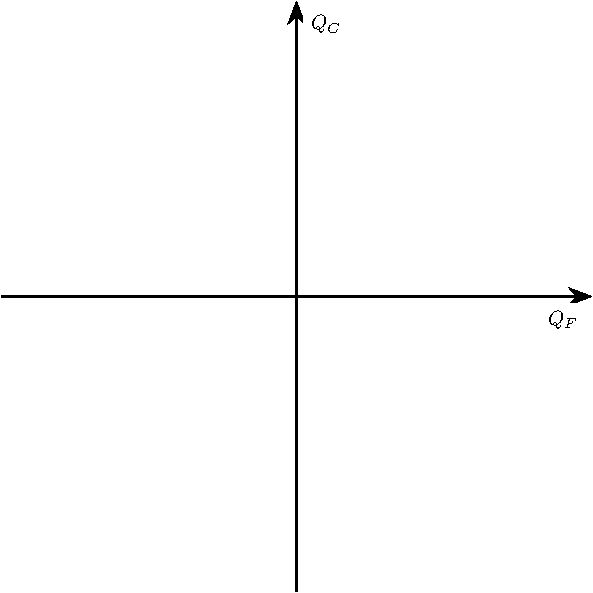
\includegraphics[width=\linewidth]{raveau-stud}
			}{
				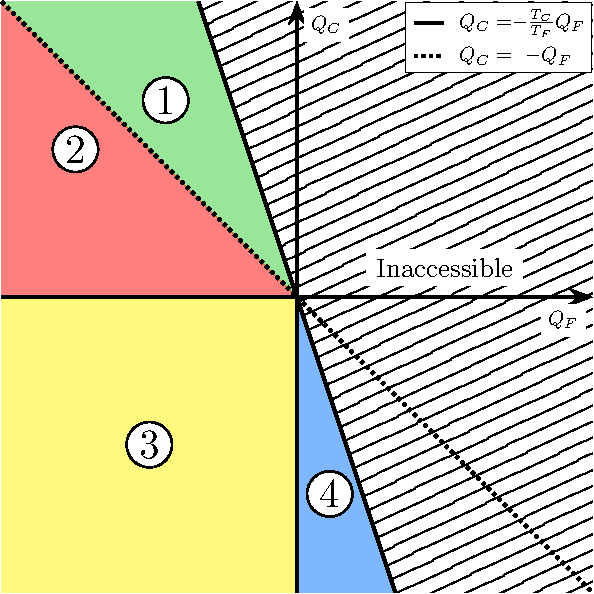
\includegraphics[width=\linewidth]{raveau}
			}
			\vspace{-15pt}
			\captionof{figure}{Diagramme de \textsc{Raveau}}
		\end{center}
	\end{isd}
\end{tcb*}

\begin{tcb*}[sidebyside, righthand ratio=.45](demo){Diagramme de \textsc{Raveau}}
	% On souhaite étudier les comportements possibles de tels systèmes, en
	% appliquant le principe de fonctionnement comme précédemment.
	On applique le principe de fonctionnement~:
	\begin{gather*}
		\beforetext{1\ier{} ppe.}
		\psw{W = -Q_C - Q_F}
		\\\beforetext{2\up{d} ppe.}
		\psw{%
			\frac{Q_C}{T_C} + \frac{Q_F}{T_F} \leq 0
			\Lra
			\boxed{Q_C \leq - \frac{T_C}{T_F} Q_F}
		}%
	\end{gather*}
	Le second principe empêche l'existence des machines ne respectant pas cette
	inégalité. De plus, pour un moteur
	\psw{%
		\begin{gather*}
			W < 0
			\Lra
			Q_F + Q_F > 0
			\Lra
			\boxed{Q_C > -Q_F}
		\end{gather*}
	}%
	Les moteurs sont au-dessus de cette droite, les autres sont récepteurs.
	\tcblower
	\begin{center}
		\sswitch{
			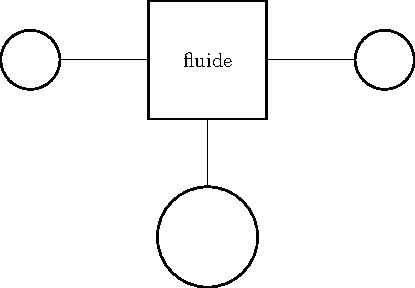
\includegraphics[width=\linewidth]{mchn_dth-stud}
		}{
			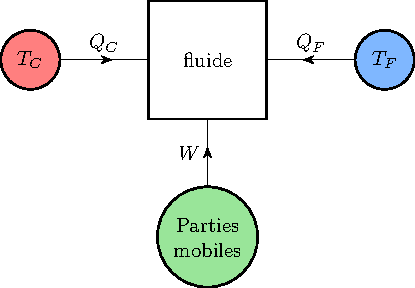
\includegraphics[width=\linewidth]{mchn_dth}
		}
		\vspace{-15pt}
		\captionof{figure}{Schéma de fonctionnement}
	\end{center}
\end{tcb*}

\begin{tcb*}(inte)<lftt>{Moteurs et réfrigérateurs}
	On peut représenter plus explicitement le fonctionnement des moteurs et
	réfrigérateurs comme suit~:
	\smallbreak
	\begin{isd}[sidebyside align=top]
		% \tcbsubtitle{\fatbox{\textbf{Moteurs}}}
		\begin{center}
			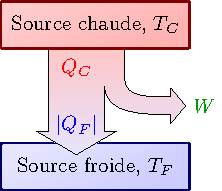
\includegraphics[height=3cm]{mot_flux}
			\captionof{figure}{Flux énergétique d'un moteur.}
		\end{center}
		\tcblower
		% \tcbsubtitle{\fatbox{\textbf{Réfrigérateurs}}}
		\begin{center}
			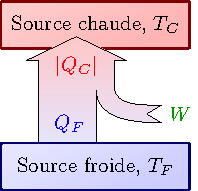
\includegraphics[height=3cm]{frig_flux}
			\captionof{figure}{Flux énergétique d'un frigo\protect\ftn{C'est aussi le
					flux d'une pompe à chaleur, en inversant qui représente la source
					froide (aliments du frigo ou air extérieur) et qui représente la
					source chaude (cuisine du frigo ou air intérieur).}.}
		\end{center}
	\end{isd}
	\vspace{-30pt}
\end{tcb*}
\vspace{-15pt}

\subsection{Moteur ditherme}
\begin{tcb*}[sidebyside](ror){Moteur ditherme}
	Domaine $\circled{1}$ du diagramme de \textsc{Raveau}~:
	\begin{gather*}
		\setlength{\fboxsep}{3mm}
		\boxed{\psw{Q_C > 0,~Q_F < 0 \text{~et~} W < 0}}
	\end{gather*}
	\begin{itemize}
		\item[b]{But}: \psw{\textbf{créer un travail}}
		\item[b]{\color{red}Source chaude}: \psw{cheminée}
		\item[b]{\color{blue}Source froide}: \psw{atmosphère}
	\end{itemize}
	\begin{tabularx}{\linewidth}{YYY}
		\textbf{Production} &
		\textbf{Coût}       &
		\textbf{Perte}
		\\
		\psw{$-W$}          &
		\psw{$Q_C$}         &
		\psw{$Q_F$}
	\end{tabularx}
	\tcblower
	\begin{center}
		\sswitch{
			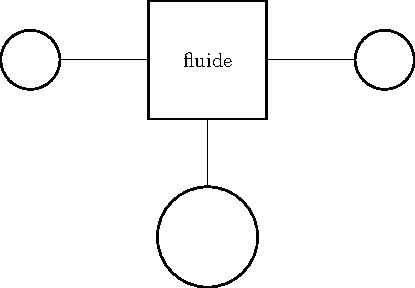
\includegraphics[width=\linewidth]{mchn_dth-stud}
		}{
			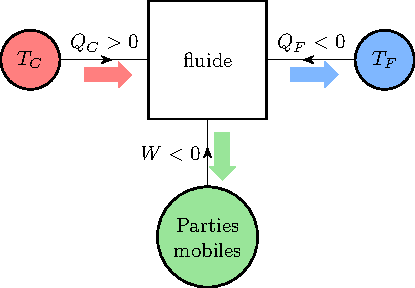
\includegraphics[width=\linewidth]{mot_dth}
		}
		\vspace{-15pt}
		\captionof{figure}{Schéma moteur ditherme.}
	\end{center}
\end{tcb*}

\begin{tcbraster}[raster equal height=rows, raster columns=2]
	\begin{tcb*}[list entry={\lte $\eta_C\sup{mot.}$}](prop){Th.\ de \textsc{Carnot}\up{mot.}}
		Il existe un cycle thermique optimal donnant un coefficient de performance
		maximal, appelé \textbf{rendement de Carnot}~:
		\psw{%
			\[
				\eta \leq \boxed{\eta_C = 1 - \frac{T_F}{T_C}}
			\]
		}%
		Il correspond au rendement idéal d'une machine réversible.
	\end{tcb*}
	\begin{tcb*}(demo)'r'{$\eta_C\sup{mot.}$}
		\psw{%
			\begin{DispWithArrows*}[fleqn, mathindent=-5pt, groups]
				% \beforetext{Rendement}
				\eta &=
				\frac{-W}{Q_C} \stc{=}{\eqref{eq:1ppe}}
				\frac{Q_C+Q_F}{Q_C}
				\\\Lra
				\eta &= 1 + \frac{Q_F}{Q_C}
				\Arrow{$\frac{Q_F}{T_F} \stc[-1]{\leq}{\eqref{eq:2ppe}} -\frac{Q_C}{T_C}$\\Or, $Q_C >
						0$\\$\frac{Q_F}{Q_C} \leq - \frac{T_F}{T_C}$}
				\\\Lra
				\eta &\leq \boxed{1 - \frac{T_F}{T_C} = \eta_C}
			\end{DispWithArrows*}
		}%
	\end{tcb*}
\end{tcbraster}

\begin{tcb*}(odgr)<lftt>{Rendement d'un moteur}
	Avec $T_C = \SI{700}{K}$ et $T_F = \SI{300}{K}$~:
	\[
		\xul{\psw{\eta_C = \num{0.6}}}
		\qet
		\xul{\psw{\eta\ind{réel} \approx \num{0.4}}}
	\]
	En pratique, les rendements observés sont de \numrange{35}{40}\,\%. En effet,
	le rendement de \textsc{Carnot} est le meilleure rendement énergétique
	possible, mais correspond à des transformations réversibles donc assez
	lentes~: la puissance fournie est faible et il faut trouver un compromis.
\end{tcb*}

\subsection{Machines frigorifiques et pompes à chaleur}
\begin{tcb*}[sidebyside](ror){Réfrigérateur}
	Domaine $\circled{4}$ du diagramme de \textsc{Raveau}~:
	\begin{gather*}
		\setlength{\fboxsep}{3mm}
		\boxed{\psw{Q_C < 0,~Q_F > 0 \text{~et~} W > 0}}
	\end{gather*}
	\begin{itemize}
		\item[b]{But}: \psw{\textbf{Refroidir une source froide}}
		\item[b]{\color{red}Source chaude}: \psw{atmosphère}
		\item[b]{\color{blue}Source froide}: \psw{aliments}
	\end{itemize}
	\begin{tabularx}{\linewidth}{YYY}
		\textbf{Production} &
		\textbf{Coût}       &
		\textbf{Perte}
		\\
		\psw{$Q_F$}         &
		\psw{$W$}           &
		\psw{$Q_C$}
	\end{tabularx}
	\tcblower
	\begin{center}
		\sswitch{
			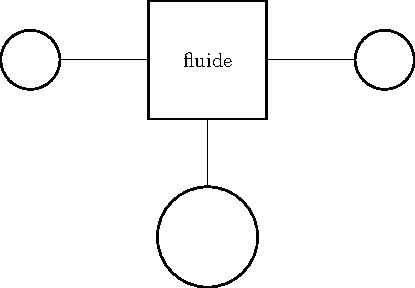
\includegraphics[width=\linewidth]{mchn_dth-stud}
		}{
			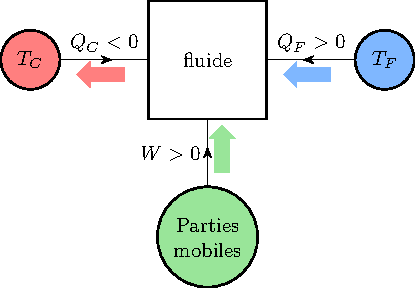
\includegraphics[width=\linewidth]{refrig_dth}
		}
		\vspace{-15pt}
		\captionof{figure}{Schéma réfrigérateur.}
	\end{center}
\end{tcb*}

\begin{tcbraster}[raster equal height=rows, raster columns=2]
	\begin{tcb*}[list entry={\lte $\eta_C\sup{frig.}$}](prop){Th.\ de \textsc{Carnot}\up{frig.}}
		Il existe un cycle thermique optimal donnant un coefficient de performance
		maximal, appelé \textbf{efficacité de Carnot}~:
		\psw{%
			\[
				e\sup{frig.} \leq \boxed{e_C\sup{frig.} = \frac{T_F}{T_C-T_F}}
			\]
		}%
		Elle correspond à l'efficacité idéale d'une machine réversible.
	\end{tcb*}
	\begin{tcb*}(demo)'r'{$e_C\sup{frig.}$}
		\psw{%
			\begin{DispWithArrows*}[fleqn, mathindent=-5pt, groups]
				e &=
				\frac{Q_F}{W} \stc{=}{\eqref{eq:1ppe}}
				-\frac{Q_F}{Q_C+Q_F}
				\\\Lra
				e &= -\frac{1}{1+\frac{Q_C}{Q_F}}
				\Arrow{$\frac{Q_C}{T_C} \stc{\leq}{\eqref{eq:2ppe}} -\frac{Q_F}{T_F}$\\Or,
					$Q_F > 0$\\$1+\frac{Q_C}{Q_F} \leq 1 - \frac{T_C}{T_F}$}
				\\\Lra
				e &\leq - \frac{1}{1 - \frac{T_C}{T_F}}
				\\\Lra
				e &\leq \boxed{\frac{T_F}{T_C-T_F} = e_C}
			\end{DispWithArrows*}
		}%
	\end{tcb*}
\end{tcbraster}

\begin{tcb*}(odgr)<lftt>{Efficacité d'un réfrigérateur}
	Avec $T_C = \SI{298}{K}$ et $T_F = \SI{278}{K}$~:
	\[
		\xul{\psw{e_C\sup{frig} = \num{13}}}
		\qet
		\xul{\psw{e\ind{réel}\sup{frig} \approx \num{3}}}
	\]
\end{tcb*}
\begin{tcb}(inte)<lftt>{Différence rendement/efficacité}
	\begin{itemize}
		\item Les coefficients de performance ont un sens plus \textbf{industriel}
		      que physique. Ceci explique qu'on puisse avoir notamment des efficacités
		      supérieures à 1. \textbf{Cela ne veut pas dire que l'on a créé de
			      l'énergie}.
		      \smallbreak
		      C'est plutôt que, dans l'énergie coûteuse, une partie n'est pas
		      directement fournie par l'utilisataire, mais implicitement donnée par
		      l'environnement.

		\item La \textbf{chaleur} est la \textbf{forme finale} de l'énergie~: tout
		      mouvement est voué à s'arrêter (à cause des frottements), en libérant
		      l'énergie sous forme de chaleur.
		      \smallbreak
		      Ainsi il est toujours beaucoup \textbf{plus simple d'extraire un transfert
			      thermique d'un travail} plutôt que l'inverse. Ce qui explique que les
		      \textbf{efficacités sont toujours plus grandes que les rendements}.
	\end{itemize}
\end{tcb}

\begin{tcb*}[sidebyside](ror){Pompe à chaleur}
	Domaine $\circled{4}$ du diagramme de \textsc{Raveau}~:
	\begin{gather*}
		\setlength{\fboxsep}{3mm}
		\boxed{\psw{Q_C < 0,~Q_F > 0 \text{~et~} W > 0}}
	\end{gather*}
	\begin{itemize}
		\item[b]{But}: \psw{\textbf{Réchauffer une source chaude}}
		\item[b]{\color{red}Source chaude}: \psw{intérieur}
		\item[b]{\color{blue}Source froide}: \psw{atmosphère}
	\end{itemize}
	\begin{tabularx}{\linewidth}{YYY}
		\textbf{Production} &
		\textbf{Coût}       &
		\textbf{Perte}
		\\
		\psw{$-Q_C$}        &
		\psw{$W$}           &
		\psw{$Q_F$}
	\end{tabularx}
	\tcblower
	\begin{center}
		\sswitch{
			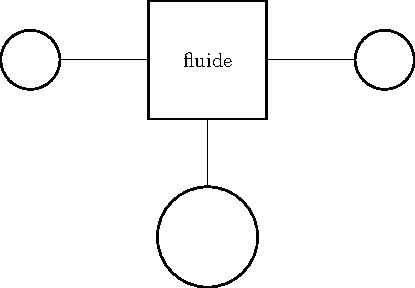
\includegraphics[width=\linewidth]{mchn_dth-stud}
		}{
			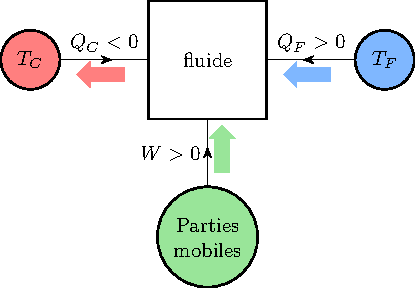
\includegraphics[width=\linewidth]{refrig_dth}
		}
		\vspace{-15pt}
		\captionof{figure}{Schéma pompe à chaleur.}
	\end{center}
\end{tcb*}

\begin{tcbraster}[raster equal height=rows, raster columns=2]
	\begin{tcb*}[list entry={\lte $\eta_C\sup{PAC}$}](prop){Th.\ de \textsc{Carnot}$\sup{PAC}$}
		Il existe un cycle thermique optimal donnant un coefficient de performance
		maximal, appelé \textbf{efficacité de Carnot}~:
		\psw{%
			\[
				e\sup{PAC} \leq \boxed{e_C\sup{PAC} = \frac{T_C}{T_C-T_F}}
			\]
		}%
		Elle correspond à l'efficacité idéale d'une machine réversible.
	\end{tcb*}
	\begin{tcb*}(demo)'r'{$e_C\sup{PAC}$}
		\psw{%
			\begin{DispWithArrows*}[fleqn, mathindent=-5pt, groups]
				e &=
				\frac{-Q_C}{W} \stc{=}{\eqref{eq:1ppe}}
				\frac{Q_C}{Q_C+Q_F}
				\\\Lra
				e &=  \frac{1}{1+\frac{Q_F}{Q_C}}
				\Arrow{$\frac{Q_F}{T_F} \stc{\leq}{\eqref{eq:2ppe}} -\frac{Q_C}{T_C}$\\Or,
					$Q_C < 0$\\$1+\frac{Q_F}{Q_C} \geq 1 - \frac{T_F}{T_C}$}
				\\\Lra
				e &\leq \frac{1}{1 - \frac{T_C}{T_F}}
				\\\Lra
				e &\leq \boxed{\frac{T_C}{T_C-T_F} = e_C}
			\end{DispWithArrows*}
		}%
	\end{tcb*}
\end{tcbraster}

\begin{tcb*}(odgr)<lftt>{Efficacité d'une pompe à chaleur}
	Avec $T_C = \SI{293}{K}$ et $T_F = \SI{278}{K}$~:
	\[
		\xul{\psw{e_C\sup{PAC} = \num{20}}}
		\qet
		\xul{\psw{e\ind{réel}\sup{PAC} \approx \num{3}}}
	\]
	L'intérêt d'une pompe à chaleur est qu'une partie de l'énergie servant à
	chauffer est prélevée dans l'environnement, et ne coûte donc rien. Son
	efficacité dépasse donc 1.
	\smallbreak
	Elle est également plus élevée que l'écart $T_C - T_F$ est petit, donc que
	l'on chauffe peu ou qu'il fasse doux dehors~: il vaut mieux garder une pompe
	allumée que de chauffer par intermittence. Comme vu dans le TDT3, \textbf{ça
		n'est pas le cas d'un radiateur} (machine monotherme).
\end{tcb*}

\section{Applications}
\subsection{Cogénération}
\begin{tcbraster}[raster equal height=rows, raster columns=2]
	\begin{tcb}(defi){Cogénération}
		La cogénération est un principe visant à valoriser toute l'énergie grâce à une
		production simultanée de plusieurs formes de puissance.
	\end{tcb}
	\begin{tcb}(exem)<rgtt>'r'{Cogénération}
		Les centrales électrique créent également beaucoup de chaleur. Il peut être
		intelligent de la récupérer afin de chauffer directement les habitations
		environnantes.
	\end{tcb}
\end{tcbraster}

\subsection{Cycle moteur de \textsc{Carnot}}
\begin{tcb*}[breakable](appl)<lftt>{Cycle moteur de \textsc{Carnot}}
	On appelle cycle de \textsc{Carnot} un cycle ditherme réversible. On considère
	une quantité $n$ de gaz parfait, et on appelle $\alpha =
		\frac{V\ind{B}}{V\ind{A}}$ subissant les transformations suivantes~:
	\begin{tasks}[label=\bdmd](2)
		\task \textbf{AB}~: détente isoT.\ quasi-statique à $T\ind{ch}$~;
		\task \textbf{BC}~: détente adia.\ réversible de $T\ind{ch}$ à $T\ind{fr}$~;
		\task \textbf{CD}~: compre$^\circ$ isoT.\ quasi-statique à $T\ind{fr}$~;
		\task \textbf{DA}~: compre$^\circ$ adia.\ réversible de $T\ind{fr}$ à
		$T\ind{ch}$.
	\end{tasks}
	% \begin{itemize}
	%   \item[b]{AB}: détente isotherme quasi-statique à $T\ind{ch}$~;
	%   \item[b]{BC}: détente adiabatique réversible de $T\ind{ch}$ à $T\ind{fr}$~;
	%   \item[b]{CD}: compression isotherme quasi-statique à $T\ind{fr}$~;
	%   \item[b]{DA}: compression adiabatique réversible de $T\ind{fr}$ à
	%     $T\ind{ch}$.
	% \end{itemize}
	\begin{enumerate}[label=\sqenumi]
		\item Tracer ce cycle en diagramme de \textsc{Watt}, en indiquant sur
		      quelles transformations il y a transfert thermique. En déduire le signe du
		      travail total. Représenter schématiquement la machine correspondante, et
		      exprimer son coefficient de performance.
		\item Exprimer $\Delta{U}\ind{AB}$, $W\ind{AB}$ et $Q\ind{AB}$ en fonction
		      de $n$, $R$, $T\ind{ch}$ et $\alpha$.
		\item Exprimer $\Delta{U}\ind{BC}$, $W\ind{BC}$ et $Q\ind{BC}$. Exprimer
		      $\frac{V\ind{C}}{V\ind{B}}$ en fonction de $T\ind{ch}$, $T\ind{fr}$ et
		      $\gamma$.
		\item Exprimer $\Delta{U}\ind{CD}$, $W\ind{CD}$ et $Q\ind{CD}$ en fonction
		      de $n$, $R$, $T\ind{fr}$, $V\ind{C}$ et $V\ind{D}$.
		\item Exprimer $\Delta{U}\ind{DA}$, $W\ind{DA}$ et $Q\ind{DA}$. Exprimer
		      $\frac{V\ind{A}}{V\ind{D}}$ en fonction de $T\ind{ch}$, $T\ind{fr}$ et
		      $\gamma$. En déduire que
		      \[
			      \alpha = \frac{V\ind{C}}{V\ind{D}}
		      \]
		      \vspace{-15pt}
		\item Par application du premier principe, déterminer alors le rendement du
		      cycle. Commenter.
		\item Déterminer l'entropie créée pour chaque transformation. Conclure.
	\end{enumerate}
	\tcblower
	\begin{enumerate}[label=\sqenumi]
		\item ~
		      \vspace{-30pt}
		      \smallbreak
		      \begin{isd}[interior hidden]
			      \sswitch{
				      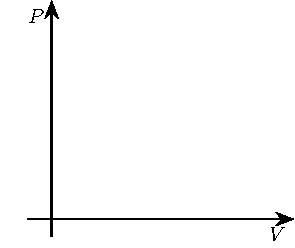
\includegraphics[width=\linewidth]{PV_carnot-stud}
			      }{
				      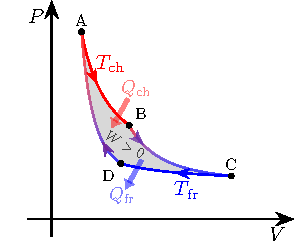
\includegraphics[width=\linewidth]{PV_carnot}
			      }
			      \vspace{-15pt}
			      \captionof{figure}{Cycle de \textsc{Carnot}.}
			      \tcblower
			      \sswitch{
				      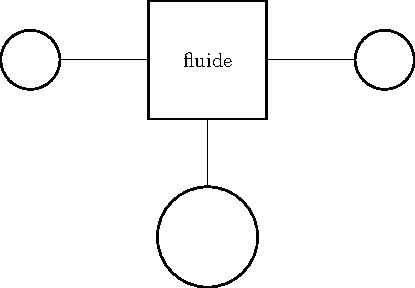
\includegraphics[width=\linewidth]{mchn_dth-stud}
			      }{
				      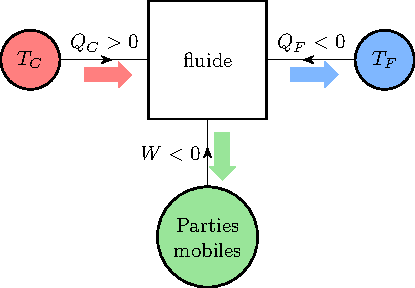
\includegraphics[width=\linewidth]{mot_dth}
			      }
			      \vspace{-15pt}
			      \captionof{figure}{Moteur ditherme.}
			      \leftcenters{%
				      On cherche
			      }{%
				      \setlength{\fboxsep}{3mm}
				      $\boxed{\psw{\DS\eta = \frac{-W}{Q_C}}}$
			      }%
			      \vspace{-15pt}
		      \end{isd}
		      \def\mspace{-25}
		\item[m]
			\begin{gather*}
				\beforetext{IsoT $\Ra$}
				\psw{%
					\Delta{T}\ind{AB} = 0
					\Lra
					\Delta{U}\ind{AB} = 0
					\Ra
					W\ind{AB} = - Q\ind{AB} = -Q\ind{ch}
				}%
				\\\beforetext{QS $\Ra$}
				\psw{%
					P = P\ind{ext} = \frac{nRT\ind{ch}}{V}
					\Ra
					\boxed{W\ind{AB} = -nRT\ind{ch}\ln \alpha = -Q\ind{ch}}
				}%
			\end{gather*}
			\vspace{\fill}
		\item[m]
			\begin{gather*}
				\beforetext{Adia $\Ra$}
				\psw{%
					Q\ind{BC} = 0
					\Ra
					\Delta{U}\ind{BC} = W\ind{BC} = C_V (T\ind{fr} - T\ind{ch})
				}%
				\\\beforetext{Rév. $\Ra$}
				\psw{%
				PV^{\gamma} = \cte
				\Lra
				TV^{\gamma-1} = \cte
				\Ra
				\boxed{\frac{V\ind{C}}{V\ind{B}} =
				\left( \frac{T\ind{ch}}{T\ind{fr}} \right)^{\frac{1}{\gamma-1}}}
				}%
			\end{gather*}
			\pagebreak
		\item[m]
			\begin{gather*}
				\beforetext{IsoT $\Ra$}
				\psw{%
					\Delta{T}\ind{CD} = 0
					\Lra
					\Delta{U}\ind{CD} = 0
					\Ra
					W\ind{CD} = - Q\ind{CD} = -Q\ind{fr}
				}%
				\\\beforetext{QS $\Ra$}
				\psw{%
					P = P\ind{ext} = \frac{nRT\ind{fr}}{V}
					\Ra
					\boxed{W\ind{CD} = -nRT\ind{fr}\ln \frac{V\ind{D}}{V\ind{C}} = -Q\ind{fr}}
				}%
			\end{gather*}
		\item[m]
			\begin{gather*}
				\beforetext{Adia $\Ra$}
				\psw{%
					Q\ind{DA} = 0
					\Ra
					\Delta{U}\ind{DA} = W\ind{DA} = C_V (T\ind{ch} - T\ind{fr})
				}%
				\\\beforetext{Rév. $\Ra$}
				% PV^{\gamma} = \cte
				% \Lra
				% TV^{\gamma-1} = \cte
				\psw{%
				\boxed{\frac{V\ind{A}}{V\ind{D}} =
				\left( \frac{T\ind{fr}}{T\ind{ch}} \right)^{\frac{1}{\gamma-1}}}
				\Lra
				\frac{V\ind{D}}{V\ind{A}} =
				\left( \frac{T\ind{ch}}{T\ind{fr}} \right)^{\frac{1}{\gamma-1}} =
				\frac{V\ind{C}}{V\ind{B}}
				\Lra
				\boxed{\frac{V\ind{B}}{V\ind{A}} = \alpha = \frac{V\ind{C}}{V\ind{D}}}
				}%
			\end{gather*}
		\item[m]
			\begin{gather*}
				\beforetext{1\ier{} ppe.}
				\psw{%
					\Delta{U}\ind{cycle} = 0
					\Lra
					W = -Q\ind{ch} - Q\ind{fr}
				}%
				\\\beforetext{Soit}
				\psw{%
					\boxed{W = nR(T\ind{fr} - T\ind{ch})\ln \alpha}
					\qet
					\boxed{Q\ind{ch} = nRT\ind{ch}\ln \alpha}
				}%
				\\\beforetext{Rendement}
				\psw{%
					\eta = \frac{-W}{Q_C}
					\Lra
					\eta = \frac{T\ind{ch}-T\ind{fr}}{T\ind{ch}}
					\Lra
					\boxed{\eta_C = 1-\frac{T\ind{fr}}{T\ind{ch}}}
				}%
			\end{gather*}
		\item[m]
			\begin{gather*}
				\beforetext{AB~:}
				\psw{%
					\Delta{S}\ind{AB} = nR \ln \frac{V\ind{B}}{V\ind{A}}
					\qet
					S\ind{ech,AB} = \frac{Q\ind{ch}}{T\ind{ch}} = nR \ln
					\frac{V\ind{B}}{V\ind{A}}
					\Lra
					\boxed{S\ind{cr,AB} = 0}
				}%
				\\\beforetext{BC~:}
				\psw{%
					\text{adia~} \Ra Q\ind{BC} = 0
					\Ra
					S\ind{ech,BC} = 0
					\qet
					\text{rév.} \Ra \boxed{S\ind{cr,BC} = 0}
					\quad \text{(BC isentropique)}
				}%
				\\\beforetext{CD~:}
				\psw{%
					\Delta{S}\ind{CD} = nR \ln \frac{V\ind{D}}{V\ind{C}}
					\qet
					S\ind{ech,CD} = \frac{Q\ind{fr}}{T\ind{fr}} = nR \ln
					\frac{V\ind{D}}{V\ind{C}}
					\Lra
					\boxed{S\ind{cr,CD} = 0}
				}%
				\\\beforetext{DA~:}
				\psw{%
					\text{adia~} \Ra Q\ind{DA} = 0
					\Ra
					S\ind{ech,DA} = 0
					\qet
					\text{rév.} \Ra \boxed{S\ind{cr,DA} = 0}
					\quad \text{(DA isentropique)}
				}%
			\end{gather*}
			\textbf{Conclusion}~: \psw{le rendement de \textsc{Carnot} correspond bien à
				une machine réversible, et est par conséquent le plus grand rendement
				possible.}
	\end{enumerate}
\end{tcb*}

\vspace{-15pt}

\subsection{Moteur à combustion~: cycle de \textsc{Beau de Rochas}}
Dans un moteur à explosion, un mélange air-carburant est enflammé et explose.
L'énergie libérée par la transformation chimique de combustion est récupérée, et
«~convertie~» sous forme de travail. Le cycle de \textbf{Beau de Rochas}\ftn{Il
	a été proposé théoriquement en 1862 par Alphonse \textsc{Beau de Rochas}. Sa
	réalisation pratique date de 1876 par Nikolaus \textsc{Otto}, en Allemagne~:
	on parle aussi du cycle d'\textsc{Otto}. En France, il a été réalisé la même
	année par Étienne \textsc{Lenoir}, qui vivait à Saint-Maur-des-Fossés~: avec
	son véhicule, il va de Joinville-le-Pont à Paris (\SI{9}{km}) en trois
	heures.} est l'un des cycles possibles d'un moteur à explosion. On peut
décomposer le cycle d'un moteur à explosion en quatre phases successives,
appelées «~temps~»\ftn{D'où le nom «~moteur 4 temps~».}, par l'étude d'un
cylindre~:

\vspace{-15pt}
\noindent
\begin{minipage}[t]{\linewidth}
	\begin{center}
		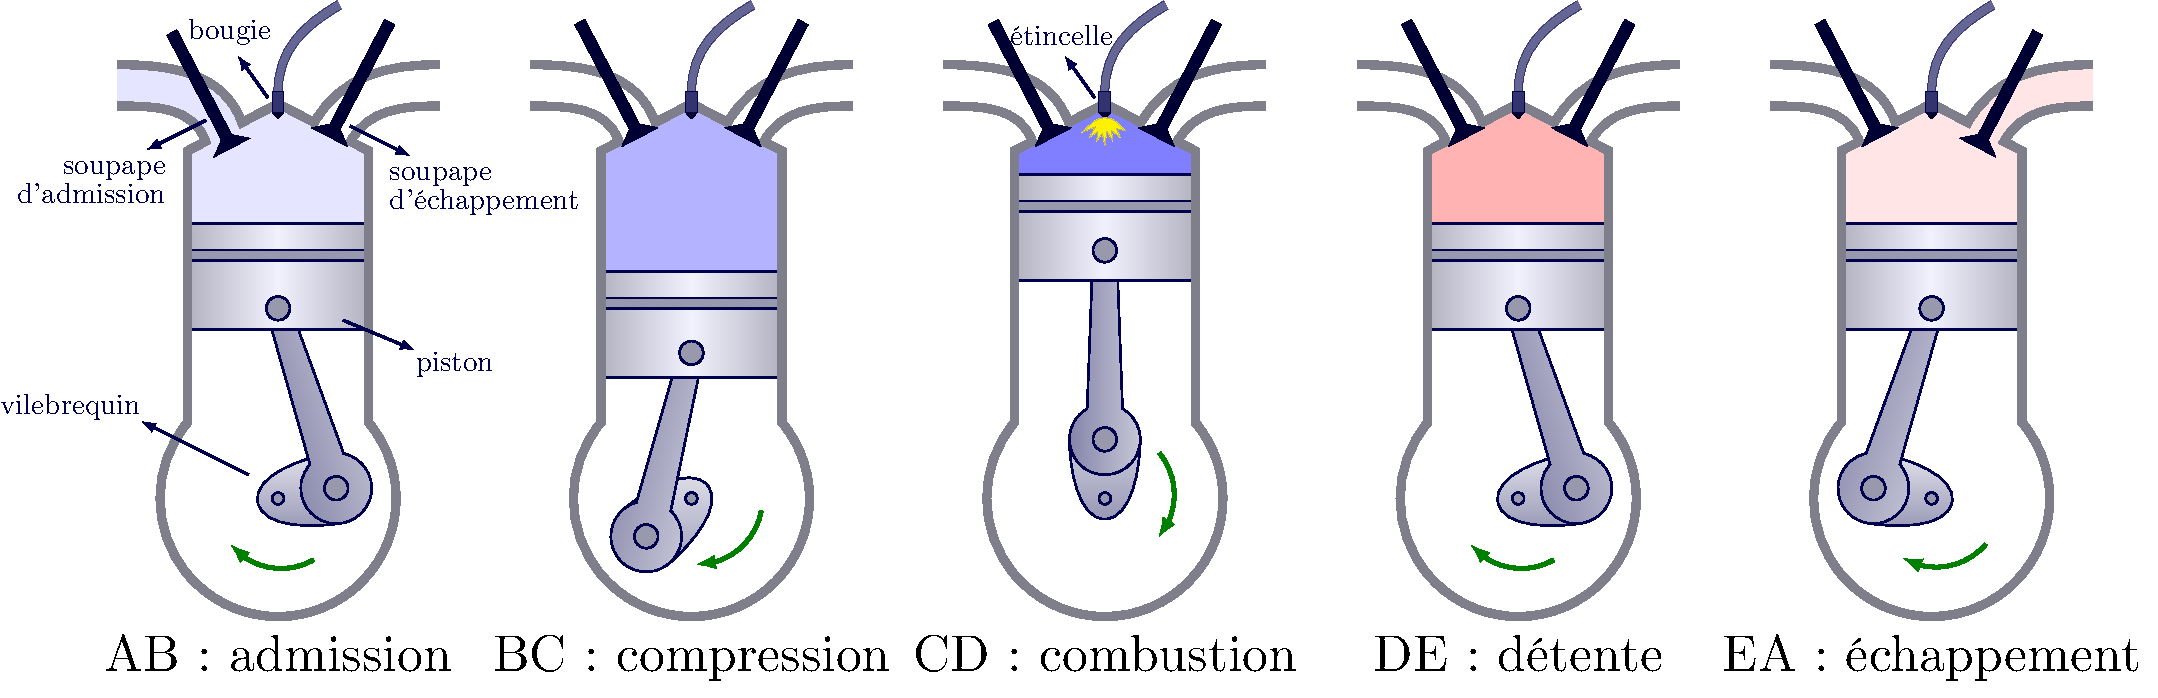
\includegraphics[width=\linewidth]{comb_bdr}
		\captionof{figure}{Cycle de transformations d'un cylindre d'un moteur à explosion.}
		\label{fig:comb_bdr}
	\end{center}
\end{minipage}

\begin{isd}
	\begin{itemize}
		\item[b]{Temps 1}: admission AB
		\smallbreak
		Le piston part de son point le plus élevé (entre E et A), de volume
		minimal, et redescend~: la soupape d'admission s'ouvre et permet le
		passage du mélange gazeux air-carburant.
		\smallbreak
		\textbf{Modèle}~: AB isobare et isotherme (mais système ouvert).
		\item[b]{Temps 2}: compression BC
		\smallbreak
		À son point le plus bas, à volume maximal, le piston remonte et la soupape
		d'admission se ferme. Le gaz est comprimé dans la chambre jusqu'à son
		volume minimal.
		\smallbreak
		\textbf{Modèle}~: BC adiabatique et réversible, donc isentropique.
		\item[b]{Temps 3}: explosion et détente CDE.
		\smallbreak
		Au volume minimal, une bougie créé une étincelle qui provoque l'explosion,
		c'est-à-dire la combustion très rapide des gaz. La pression augmente
		fortement. Le gaz ainsi chauffé repousse violemment le piston vers le
		bas~: c'est le \textbf{temps moteur}, où du travail est effectivement
		reçu par le piston. Il redescend jusqu'à son volume maximal.
		\smallbreak
		\textbf{Modèle}~: explosion CD rapide, donc isochore, et détente DE
		isentropique.
		\item[b]{Temps 4}: échappement EA.
		\smallbreak
		Au point E, la soupape d'échappement s'ouvre sur l'atmosphère et le piston
		remonte vers le point A en expulsant les gaz brûlés. La soupape
		d'échappement se ferme alors, celle d'admission s'ouvre, on revient au
		premier temps.
		\smallbreak
		\textbf{Modèle}~: EA isobare et isotherme, mais système ouvert.
	\end{itemize}
	\tcblower
	\begin{center}
		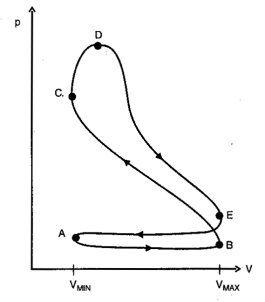
\includegraphics[width=\linewidth]{cycle_bdr}
		\captionof{figure}{Cycle réel.}
	\end{center}
	\begin{center}
		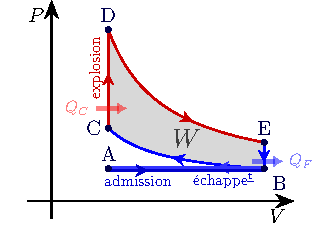
\includegraphics[width=\linewidth]{PV_otto}
		\captionof{figure}{Cycle idéal.}
	\end{center}
\end{isd}

\subsection{Autres machines}
\begin{itemize}
	\item Moteur diesel~: compression adiabatique, chauffage isobare, détente
	      adiabatique, refroidissement isochore~;
	\item Moteur \textsc{Stirling} (voir TD)~: deux isothermes, deux
	      isochores~;
	\item La turbine à gaz, modélisée par le cycle de \textsc{Joule-Brayton}~:
	      deux adiabatiques, deux isobares.
\end{itemize}
Le réfrigérateur et la pompe à chaleur font intervenir des changements d'états
et des systèmes ouvert~: on y reviendra au prochain chapitre.

\end{document}

% \begin{center}
% 	\begin{tikzpicture}[scale=1.3]
% 		\draw [->](0,0) -- (0,3.5) node[anchor=west]{$P$};
% 		\draw [->](0,0) -- (5.5,0) node[anchor=west]{$V$};
%
% 		\draw[dashed] plot [domain=0.8:5] (\x,3/\x) node[below]{$T_f$};
% 		\draw[very thick, red,simplef] plot [domain=1.5:3] (\x,3/\x);
% 		\draw[very thick, red,simplef] plot [domain=1.0203:1.5] (\x,{3.5282/(\x^(1.4))});
% 		\draw[dashed] plot [domain=0.8:5] (\x,3.5/\x) node[above]{$T_c$};
% 		\draw[very thick, red,simplef] plot [domain=2.0406:1.0203] (\x,3.5/\x);
% 		\draw[very thick, red,simplef] plot [domain=3:2.0406] (\x,{4.6555/(\x^(1.4))});
%
% 		\fill (3,1) circle(0.04);
% 		\fill (1.5,2) circle(0.04);
% 		\fill (1.0203,3.43) circle(0.04);
% 		\fill (2.0406,1.72) circle(0.04);
%
% 		\node[above] at (3,1) {A};
% 		\node[left] at (1.5,2) {D};
% 		\node[right] at (1.0203,3.43) {C};
% 		\node[right] at (2.0406,1.72) {B};
% 	\end{tikzpicture}
% \end{center}
